% Options for packages loaded elsewhere
\PassOptionsToPackage{unicode}{hyperref}
\PassOptionsToPackage{hyphens}{url}
\PassOptionsToPackage{dvipsnames,svgnames,x11names}{xcolor}
\documentclass[
  11pt,
  a4paper,
]{article}
\usepackage{xcolor}
\usepackage[margin=24mm]{geometry}
\usepackage{amsmath,amssymb}
\setcounter{secnumdepth}{-\maxdimen} % remove section numbering
\usepackage{iftex}
\ifPDFTeX
  \usepackage[T1]{fontenc}
  \usepackage[utf8]{inputenc}
  \usepackage{textcomp} % provide euro and other symbols
\else % if luatex or xetex
  \usepackage{unicode-math} % this also loads fontspec
  \defaultfontfeatures{Scale=MatchLowercase}
  \defaultfontfeatures[\rmfamily]{Ligatures=TeX,Scale=1}
\fi
\usepackage{lmodern}
\ifPDFTeX\else
  % xetex/luatex font selection
  \setmainfont[BoldFont=texgyrepagella-bold.otf,ItalicFont=texgyrepagella-italic.otf,BoldItalicFont=texgyrepagella-bolditalic.otf]{texgyrepagella-regular.otf}
  \setmonofont[BoldFont=lmmonolt10-bold.otf]{lmmono10-regular.otf}
  \setmathfont[]{texgyrepagella-math.otf}
\fi
% Use upquote if available, for straight quotes in verbatim environments
\IfFileExists{upquote.sty}{\usepackage{upquote}}{}
\IfFileExists{microtype.sty}{% use microtype if available
  \usepackage[]{microtype}
  \UseMicrotypeSet[protrusion]{basicmath} % disable protrusion for tt fonts
}{}
\makeatletter
\@ifundefined{KOMAClassName}{% if non-KOMA class
  \IfFileExists{parskip.sty}{%
    \usepackage{parskip}
  }{% else
    \setlength{\parindent}{0pt}
    \setlength{\parskip}{6pt plus 2pt minus 1pt}}
}{% if KOMA class
  \KOMAoptions{parskip=half}}
\makeatother
\usepackage{graphicx}
\makeatletter
\newsavebox\pandoc@box
\newcommand*\pandocbounded[1]{% scales image to fit in text height/width
  \sbox\pandoc@box{#1}%
  \Gscale@div\@tempa{\textheight}{\dimexpr\ht\pandoc@box+\dp\pandoc@box\relax}%
  \Gscale@div\@tempb{\linewidth}{\wd\pandoc@box}%
  \ifdim\@tempb\p@<\@tempa\p@\let\@tempa\@tempb\fi% select the smaller of both
  \ifdim\@tempa\p@<\p@\scalebox{\@tempa}{\usebox\pandoc@box}%
  \else\usebox{\pandoc@box}%
  \fi%
}
% Set default figure placement to htbp
\def\fps@figure{htbp}
\makeatother
\setlength{\emergencystretch}{3em} % prevent overfull lines
\providecommand{\tightlist}{%
  \setlength{\itemsep}{0pt}\setlength{\parskip}{0pt}}
\usepackage{mathtools}
\usepackage{graphicx}
\usepackage{needspace}
\usepackage{xurl}
\usepackage{etoolbox}
\usepackage{fancyhdr}
\usepackage{titlesec}
\setlength{\parindent}{0pt}
\setlength{\parskip}{5.5pt plus 1pt minus 1pt}
\setlength{\emergencystretch}{2em}
\clubpenalty=10000
\widowpenalty=10000
\displaywidowpenalty=10000
\raggedbottom
\pagestyle{fancy}
\fancyhf{}
\fancyfoot[C]{\small\thepage}
\renewcommand{\headrulewidth}{0pt}
\titleformat{\section}{\normalfont\Large\bfseries}{}{0pt}{}
\titlespacing*{\section}{0pt}{16pt plus 3pt minus 2pt}{7pt}
\pretocmd{\section}{\Needspace{6\baselineskip}}{}{}
\makeatletter
\renewenvironment{figure}[1][]{\par\noindent\begin{minipage}{\linewidth}\def\@captype{figure}}{\end{minipage}\par\medskip}
\def\@maketitle{%
 \newpage\null\vskip 0.1em
 \begin{center}{\LARGE\bfseries\@title\par}\vskip 0.9em
 {\large\@author\par}\vskip 0.25em
 {\small\href{mailto:pzychozen@gmail.com}{pzychozen@gmail.com}\par}
 \vskip 0.35em{\small\@date\par}\end{center}\par\vskip 0.5em}
\makeatother
\newsavebox{\papereqbox}
\newcommand{\paperdisplay}[2][]{%
 \par\begingroup
 \sbox{\papereqbox}{$\displaystyle #2$}%
 \typeout{PAPER-EQUATION-WIDTH: \the\wd\papereqbox; available \the\linewidth; tag #1}%
 \begin{equation*}
 \ifdim\wd\papereqbox>.90\linewidth
 \resizebox{.90\linewidth}{!}{\usebox{\papereqbox}}%
 \else\usebox{\papereqbox}\fi
 \ifstrempty{#1}{}{\tag{#1}}
 \end{equation*}\endgroup\par}
\usepackage{bookmark}
\IfFileExists{xurl.sty}{\usepackage{xurl}}{} % add URL line breaks if available
\urlstyle{same}
% fallback for those not using the hyperref driver hyperxmp:
\makeatletter
\@ifundefined{xmpquote}{\newcommand{\xmpquote}[1]{#1}}{}
\makeatother
\hypersetup{
  pdftitle={Triadic Chirality and Orientation Geometry},
  pdfauthor={Hilmir Frímann Halldórsson},
  colorlinks=true,
  linkcolor={MidnightBlue},
  filecolor={Maroon},
  citecolor={Blue},
  urlcolor={MidnightBlue},
  pdfcreator={LaTeX via pandoc}}

\title{Triadic Chirality and Orientation Geometry}
\author{Hilmir Frímann Halldórsson}
\date{Draft v0.1 - 23 September 2026}

\begin{document}
\maketitle

\subsection{Abstract}\label{abstract}

A complex three-channel state has an exact realization as three tangent vectors on a folded module of regular octagons. We specify the outward-oriented face frames and a matched, zero-relative-phase transport between their tangent planes. The resulting encoding is a real isometry and a complex-linear identification once each plane is equipped with its outward-normal complex structure. Transport preserves the two components, composes exactly, and agrees with the appropriate cyclic spatial rotation on its tangent domain. The existing nonlinear triad recurrence consequently admits an exact expression in these geometric coordinates. Our main identity identifies the raw channel chirality \(\operatorname{Re}\Omega\times\operatorname{Im}\Omega\) with a cyclic triple of transported signed areas. We derive its spatial and channel transformation laws, including the two distinct determinant factors under reflections and relabellings. An explicit cyclic-rotation witness separates this channel pseudovector from an ambient axial vector. The construction is finite-dimensional and kinematic: adopting tangent vectors as the state observable does not supply a physical field, seam law, units, or time scale.

\subsection{1. A geometric meaning for a complex triad}\label{a-geometric-meaning-for-a-complex-triad}

Let \(\Omega=(\Omega_A,\Omega_B,\Omega_C)^T\in\mathbb C^3\) be a raw, unnormalized state. Its three complex entries can be attached to the faces of a folded three-octagon module, but attachment by labels alone does not explain what their real and imaginary parts mean geometrically. Nor does a cross product of their three real and three imaginary coordinates automatically produce a vector in physical space. These are different questions about different vector spaces.

We answer the first question by selecting the oriented tangent plane at each face centre. Each plane has two real coordinates, an outward normal and a Euclidean complex structure. A common vertical axis fixes a coherent frame on all three planes. This choice turns complex amplitudes into tangent vectors without changing their scale. It also makes it possible to compare vectors on different faces through an explicit transport. The second question is then answered by identifying channel chirality with three signed, transported state-vector areas and deriving the representation under which that triple transforms.

The geometry is the width-one folded shell of {[}PC{]}. The recurrence is the three-node map of {[}PA{]}. The tangent-space construction and its compatible area form were established in the geometry-to-state bridge and its corrected second-stage analysis {[}BI, BII{]}; the completed face-state attachment specifies their use as a geometric view {[}FA{]}. Here those ingredients are assembled into a self-contained argument with the ambient/tangent and spatial/channel distinctions made explicit. We claim a precise realization of this model, not novelty for the underlying complex-plane or alternating-form identities.

Statements below identify their provenance. ``Reused'' means that the underlying result is taken from the named source, with enough algebra supplied here to fix conventions. ``Adopted'' marks the modelling choice of a state observable or transport convention. Neither label is a physical derivation. All statements concern the local module shown in Figure 1.

\begin{figure}
\centering
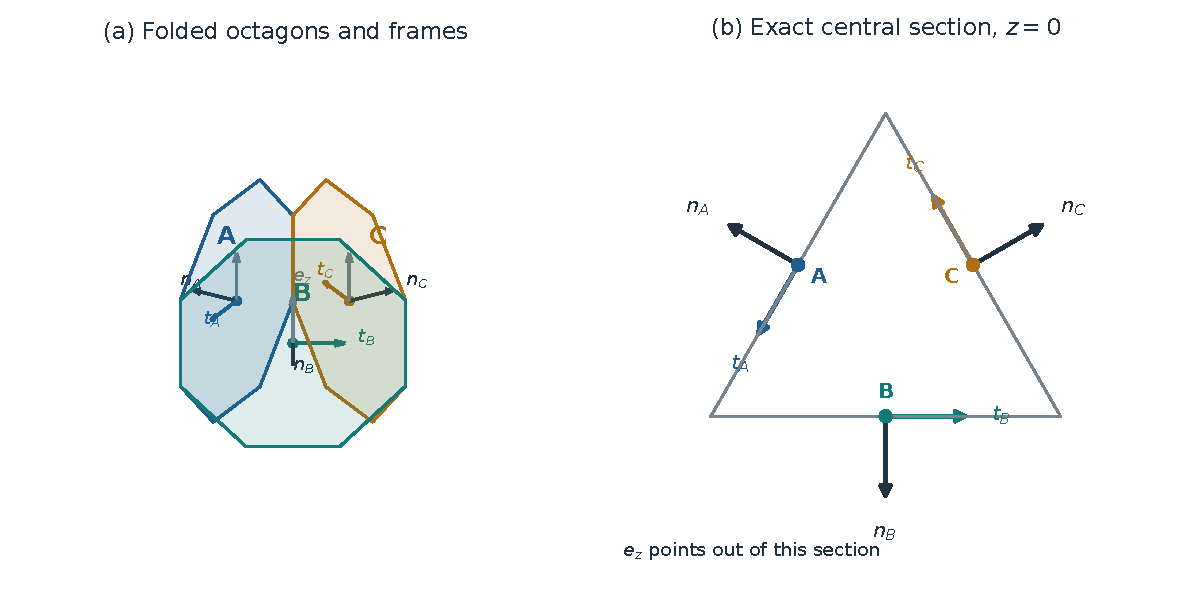
\includegraphics[width=1\linewidth,height=\textheight,keepaspectratio,alt={Exact width-one folded module. The left panel shows the three octagons; the right panel is the central section in the horizontal plane with the same face centres, outward normals and tangent directions. Frame arrows have a common display scale; their mathematical vectors are unit vectors. The vertical direction is common to all faces.}]{figures/figure_1_folded_frames.pdf}
\caption{Exact width-one folded module. The left panel shows the three octagons; the right panel is the central section in the horizontal plane with the same face centres, outward normals and tangent directions. Frame arrows have a common display scale; their mathematical vectors are unit vectors. The vertical direction is common to all faces.}
\end{figure}

\subsection{2. Exact folded orientation geometry}\label{exact-folded-orientation-geometry}

Write \(s=\sqrt2-1\) and let the local material octagon have vertices, in order,
\paperdisplay[1]{\begin{aligned}
&(-\tfrac12,-\tfrac s2),\ (-\tfrac s2,-\tfrac12),\
(\tfrac s2,-\tfrac12),\ (\tfrac12,-\tfrac s2),\\
&(\tfrac12,\tfrac s2),\ (\tfrac s2,\tfrac12),\
(-\tfrac s2,\tfrac12),\ (-\tfrac12,\tfrac s2).
\end{aligned}}
The coordinates are \((u,z)\). The accepted placement is
\paperdisplay[2]{\begin{aligned}
X_A(u,z)&=(-\tfrac14-\tfrac u2,\ \tfrac{\sqrt3}{4}-\tfrac{\sqrt3 u}{2},\ z),\\
X_B(u,z)&=(u,0,z),\\
X_C(u,z)&=(\tfrac14-\tfrac u2,\ \tfrac{\sqrt3}{4}+\tfrac{\sqrt3 u}{2},\ z).
\end{aligned}}
These isometric panel maps, their welded shell and outward orientations are reused from {[}PC, §§4, 5, 7, 9{]}. The shell has three faces and two boundary rims; its topology is that of an annulus. We use its geometry only as a carrier for three selected tangent spaces. No field is extended over the shell in this construction.

The face centres, outward unit normals and horizontal tangent vectors are
\paperdisplay[3]{\begin{aligned}
c_A&=(-\tfrac14,\tfrac{\sqrt3}{4},0),&
n_A&=(-\tfrac{\sqrt3}{2},\tfrac12,0),&
t_A&=(-\tfrac12,-\tfrac{\sqrt3}{2},0),\\
c_B&=(0,0,0),&
n_B&=(0,-1,0),&
t_B&=(1,0,0),\\
c_C&=(\tfrac14,\tfrac{\sqrt3}{4},0),&
n_C&=(\tfrac{\sqrt3}{2},\tfrac12,0),&
t_C&=(-\tfrac12,\tfrac{\sqrt3}{2},0).
\end{aligned}}
With \(e_z=(0,0,1)\), these satisfy
\paperdisplay[4]{t_i=e_z\times n_i,\qquad t_i\times e_z=n_i,\qquad
n_i\times t_i=e_z,\qquad n_i\times e_z=-t_i.}
Thus \((t_i,e_z)\) is the positive orthonormal basis of the \(i\)th plane. Once the outward normal and positive vertical direction are fixed, there is no remaining choice of \(t_i\) in this convention. In particular, a \(45^\circ\) rotation of an isolated regular octagon is not a symmetry of the entire welded shell.

Let \(o=(0,\sqrt3/6,0)\) and define
\paperdisplay[5]{R=\begin{pmatrix}
-1/2&-\sqrt3/2&0\\
\sqrt3/2&-1/2&0\\
0&0&1
\end{pmatrix},\qquad
P=\begin{pmatrix}0&0&1\\1&0&0\\0&1&0\end{pmatrix}.}
The spatial \(C_3\) generator is the affine map \(x\mapsto o+R(x-o)\); it sends \(A\) to \(B\), \(B\) to \(C\), and \(C\) to \(A\). Its action on free vectors is \(R\). The matrix \(P\) acts on ordered channel triples, so \((P\Omega)_B=\Omega_A\).

Two useful mirrors are \(H=\operatorname{diag}(1,1,-1)\) and \(V=\operatorname{diag}(-1,1,1)\). The first fixes every face label; the second swaps \(A\) and \(C\) and fixes \(B\). Together with the cyclic rotation these generate the unlabelled shell\textquotesingle s \(D_{3h}\) point group {[}PC{]}. The notation is the standard Schoenflies convention {[}Cotton90, AH94{]}. Point-group language describes the geometry; it does not yet assert a dynamical symmetry.

\subsection{3. Three oriented planes as a complex state space}\label{three-oriented-planes-as-a-complex-state-space}

Let \(W_i=n_i^\perp\subset\mathbb R^3\) denote the vector plane attached at \(c_i\), and let \(W_{\mathrm{tan}}=W_A\oplus W_B\oplus W_C\). These are planes of free vectors, not bounded polygonal faces: a vector may have any magnitude and its endpoint need not lie inside an octagon.

\textbf{Adoption 1 (state observable).} We represent \(\Omega_i=q_i+\mathrm i p_i\) by
\paperdisplay[6]{D_i(\Omega_i)=v_i=q_i t_i+p_i e_z,\qquad
E_i(v_i)=t_i\cdot v_i+\mathrm i\,e_z\cdot v_i.}
Write \(D=\bigoplus_iD_i\) and \(E=\bigoplus_iE_i\). Selecting these vectors as the model\textquotesingle s observable is the adoption made in {[}FA, §§3, 10{]}. It does not assert that the vectors are a recovered physical field.

\textbf{Proposition 1 (oriented complex planes; reused from {[}BI, BII{]}, with exact verification).} On \(W_i\), the operator \(J_i v=n_i\times v\) satisfies \(J_i^2=-I\), is orthogonal, and obeys \(E_i(J_i v)=\mathrm i E_i(v)\). The maps \(D\) and \(E\) are inverse real isometries between \(\mathbb C^3\) and \(W_{\mathrm{tan}}\), and become complex-linear for the structures \(\mathrm i\) and \(J=\bigoplus_iJ_i\).

\emph{Proof.} Equation (4) gives \(J_i(qt_i+pe_z)=-pt_i+qe_z\), the coordinate rule for multiplication by \(\mathrm i\). A second application changes both signs. Orthonormality gives \(\|v_i\|^2=q_i^2+p_i^2=|\Omega_i|^2\) and the inverse formula (6). Summing over faces proves the isometry. On the ambient space \((\mathbb R^3)^3\), the same formula for \(DE\) is instead the block tangent projector,
\paperdisplay[7]{\Pi_i=t_i t_i^T+e_z e_z^T=I-n_i n_i^T.}
It is not the nine-dimensional identity. \(\square\)

\begin{figure}
\centering
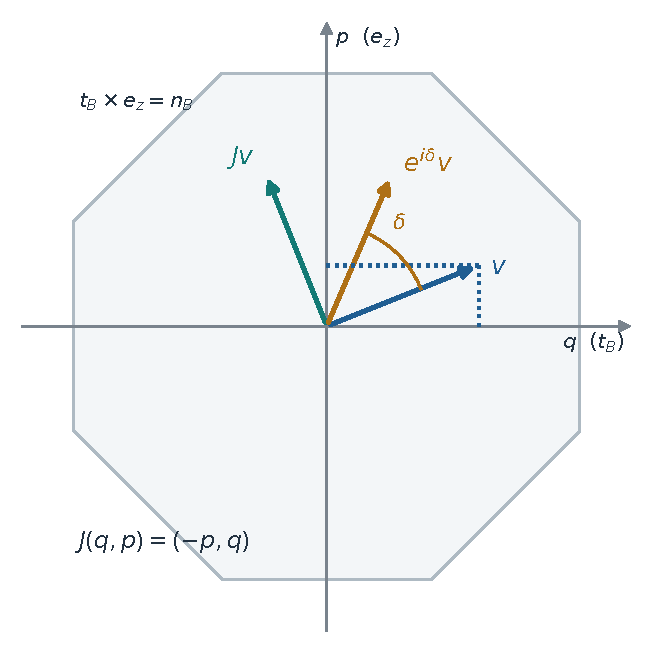
\includegraphics[width=0.72\linewidth,height=\textheight,keepaspectratio,alt={Face B in its exact oriented coordinates. The sample vector has coordinates (0.30,0.12); J rotates it through a positive right angle, and multiplication by \textbackslash exp(\textbackslash mathrm i\textbackslash delta) gives the displayed rotation with \textbackslash delta=\textbackslash pi/4. The outline is the actual width-one octagon. All arrows lie in the tangent plane; the outward normal points toward the reader.}]{figures/figure_2_complex_plane.pdf}
\caption{Face B in its exact oriented coordinates. The sample vector has coordinates \((0.30,0.12)\); \(J\) rotates it through a positive right angle, and multiplication by \(\exp(\mathrm i\delta)\) gives the displayed rotation with \(\delta=\pi/4\). The outline is the actual width-one octagon. All arrows lie in the tangent plane; the outward normal points toward the reader.}
\end{figure}

The compatible bilinear forms are
\paperdisplay[8]{g_i(v,w)=v\cdot w,\qquad
\omega_i(v,w)=n_i\cdot(v\times w)=g_i(J_i v,w).}
In coordinates, \(\omega_i=dq_i\wedge dp_i\) and its matrix is
\(\begin{pmatrix}0&1\\-1&0\end{pmatrix}=-[J_i]\).
This sign matters: the matrix of the form is not the matrix of the complex structure. The identity \(\omega_i(v,J_iw)=g_i(v,w)\) fixes compatibility. The form is nondegenerate and constant, hence closed. With the constant complex structure this is a flat Kähler plane, and the direct sum gives the corresponding flat structure on \(W_{\mathrm{tan}}\) {[}BII{]}. The assertion is about the selected vector space; it is not a claim of a smooth Kähler structure across the creases of the shell.

\subsection{4. Matched transport between faces}\label{matched-transport-between-faces}

Vectors on distinct faces lie in different tangent planes. Comparing their components requires an identification of these planes.

\textbf{Adoption 2 (zero-relative-phase transport).} Use the common frames of (3) and set
\paperdisplay[9]{T_{ij}=t_i t_j^T+e_z e_z^T,
\qquad T_{ij}: \mathbb R^3\longrightarrow\mathbb R^3.}
The first index is the destination and the second the source. This fixes the same \(q,p\) components in both frames and inserts no extra relative phase. The convention is the one implemented in {[}FA, §10{]}.

\textbf{Proposition 2 (transport identities; inherited from {[}FA, §10{]}, proved here).} The restriction of \(T_{ij}\) to \(W_j\) is a complex-linear isometry onto \(W_i\). As ambient matrices,
\paperdisplay[10]{T_{ij}T_{jk}=T_{ik},\qquad
T_{ii}=\Pi_i,\qquad
T_{ij}=\Pi_i R_{ij},}
where \(R_{ij}\) is the linear part of the unique element of the threefold rotation group taking face \(j\) to face \(i\).

\emph{Proof.} Directly,
\(T_{ij}(q t_j+p e_z)=q t_i+p e_z\), so components, norm and \(J\) are preserved. Multiplying the outer products in (9), the two mixed terms vanish and the two diagonal terms have scalar factor one. This proves composition on all of \(\mathbb R^3\), including normal inputs. Equation (7) gives \(T_{ii}\). Finally \(R_{ij}\) takes \((t_j,e_z,n_j)\) to \((t_i,e_z,n_i)\); following it with \(\Pi_i\) removes the last component and yields (9). \(\square\)

Each \(T_{ij}\) has rank two and kills \(n_j\). It is therefore not a full ambient rigid rotation, although its tangent restriction agrees with \(R_{ij}\). Likewise, moving an attached point \(c_j+v\) requires the affine rotation about the centroid axis; transporting the free vector \(v\) uses the linear action. Confusing those operations would rotate the centres about the wrong axis.

\begin{figure}
\centering
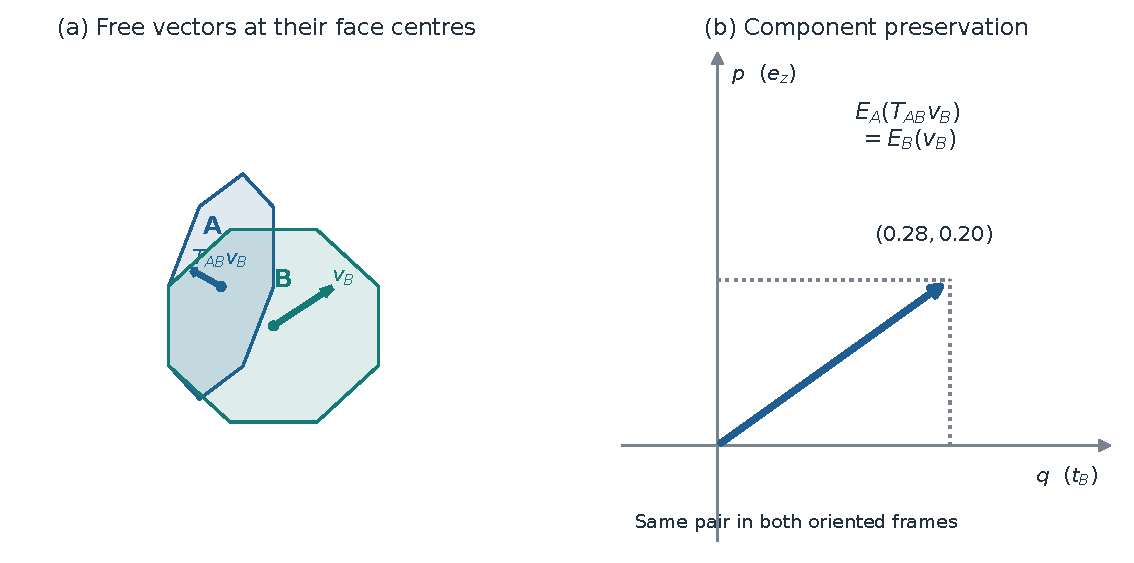
\includegraphics[width=1\linewidth,height=\textheight,keepaspectratio,alt={Transport from face B to face A. The left panel uses the exact face placements and a vector with q=0.28, p=0.20. Its image has the same two components at the destination centre. The right panel displays the shared component pair; it is a coordinate comparison, not a flattening of the welded shell.}]{figures/figure_3_transport.pdf}
\caption{Transport from face B to face A. The left panel uses the exact face placements and a vector with \(q=0.28\), \(p=0.20\). Its image has the same two components at the destination centre. The right panel displays the shared component pair; it is a coordinate comparison, not a flattening of the welded shell.}
\end{figure}

This transport identifies three specified vector spaces. It gives neither a field trace across a seam nor a rule for moving along arbitrary paths on the surface. In particular, the composition identity in (10) does not supply a physical connection or a seam-continuity condition.

\subsection{5. The existing triad law in geometric coordinates}\label{the-existing-triad-law-in-geometric-coordinates}

We now express the map of {[}PA, §6.1{]} in these coordinates. Take real parameters \(\varepsilon,g,\lambda\) and \(k=(k_A,k_B,k_C)\in\mathbb R^3\). With entrywise multiplication denoted by \(\odot\), its pre-synchronization step is
\paperdisplay[11]{\widetilde\Omega=\Omega+\varepsilon\,\Omega\odot(k-|\Omega|^2)+gL_3\Omega,
\qquad
L_3=\begin{pmatrix}-2&1&1\\1&-2&1\\1&1&-2\end{pmatrix}.}
The phase step uses
\paperdisplay[12]{\begin{aligned}
\phi_i&=\operatorname{Arg}_0(\widetilde\Omega_i),&
\operatorname{Arg}_0(z)&=\begin{cases}\arg z,&z\ne0,\\0,&z=0,\end{cases}\\
\delta_i&=\lambda\sum_{j\ne i}\sin\bigl(3(\phi_j-\phi_i)\bigr),&
\Omega_i^+&=|\widetilde\Omega_i|\exp\bigl(\mathrm i(\phi_i+\delta_i)\bigr).
\end{aligned}}
All increments are evaluated simultaneously from \(\widetilde\Omega\). If \(\lambda=0\), the phase step is defined directly as the identity. Denote this whole map by \(F_{\mathrm{TO}}\).

\textbf{Theorem 3 (coordinate conjugacy; reused from {[}PA{]} and {[}FA{]}, with exact derivation).} On \(W_{\mathrm{tan}}\), the corresponding pre-synchronization step is
\paperdisplay[13]{\widetilde v_i=
v_i+\varepsilon(k_i-\|v_i\|^2)v_i
+g\sum_{j\ne i}(T_{ij}v_j-v_i).}
The full geometric map is
\paperdisplay[14]{F_{\mathrm{face}}=D F_{\mathrm{TO}} E,\qquad
v_i^+=\cos\delta_i\,\widetilde v_i+\sin\delta_i\,J_i\widetilde v_i.}

\emph{Proof.} Proposition 1 identifies \(\|v_i\|^2\) with \(|\Omega_i|^2\). Proposition 2 gives \(E_i(T_{ij}v_j)=\Omega_j\). Encoding (13) therefore yields exactly the \(i\)th component of (11). The identity \(E_iJ_i=\mathrm i E_i\) turns the second formula of (14) into multiplication by \(\exp(\mathrm i\delta_i)\). Since \(\widetilde v_i\) already encodes the phase \(\phi_i\) when nonzero, this is (12). If it is zero, rotation and amplitude reconstruction both return zero. The equality holds on the entire stated domain with the same zero convention. \(\square\)

Equation (14) is a coordinate conjugacy, not an independent evolution law or a new force. In particular, the geometry does not derive the cubic amplitude term, the coupling coefficient, the harmonic three, or a clock. These are inputs of the already specified recurrence.

For nonzero pre-synchronization components, a common phase shift cancels from every phase difference. At \(\lambda\ne0\), the assignment \(\operatorname{Arg}_0(0)=0\) prevents that argument from being extended indiscriminately to the zero stratum: a zero vector has no direction, yet its assigned phase enters its neighbours\textquotesingle{} increments. The extension is generally discontinuous there {[}PA{]}. The conjugacy remains valid because it carries the same convention, not because it removes that convention. Section 9 states the parameter qualifications separately.

\subsection{6. Chirality as transported signed area}\label{chirality-as-transported-signed-area}

The real and imaginary channel vectors are \(a=\operatorname{Re}\Omega\) and \(b=\operatorname{Im}\Omega\). Their raw channel cross product is
\(Z_{\mathrm{chiral}}(\Omega)=a\times b\).
We write \(Z\) for this observable. Its three entries refer to ordered channel pairs; the following theorem identifies their geometric content.

\Needspace{14\baselineskip}

\textbf{Theorem 4 (transported area; inherited from {[}BII, FA{]}, with a self-contained proof).} Define
\paperdisplay[15]{\mathcal A_{ij}=n_i\cdot\bigl[v_i\times(T_{ij}v_j)\bigr].}
Then
\paperdisplay[16]{\begin{aligned}
\mathcal A_{ij}
&=q_i p_j-p_i q_j
=\operatorname{Im}(\overline{\Omega_i}\Omega_j)
=\omega_i(v_i,T_{ij}v_j),\\
Z&=(\mathcal A_{BC},\mathcal A_{CA},\mathcal A_{AB})^T
=a\times b .
\end{aligned}}
In particular \(\mathcal A_{ji}=-\mathcal A_{ij}\), \(\mathcal A_{ii}=0\), and multiplication of the whole state by \(c\in\mathbb C\) multiplies every area and \(Z\) by \(|c|^2\).

\emph{Proof.} The two vectors in (15), expressed at face \(i\), are \(q_i t_i+p_i e_z\) and \(q_j t_i+p_j e_z\). Bilinearity of the cross product and \(t_i\times e_z=n_i\) give
\((q_i p_j-p_i q_j)n_i\). Taking the normal component proves the first formula. The imaginary part of \((q_i-\mathrm i p_i)(q_j+\mathrm i p_j)\) is the same determinant. Listing the three cyclic pairs gives the defining coordinates of \(a\times b\). Antisymmetry and the zero diagonal follow by exchanging equal or distinct indices. Finally \(\overline{c\Omega_i}\,c\Omega_j=|c|^2\overline{\Omega_i}\Omega_j\). \(\square\)

Thus \(\mathcal A_{ij}\) is the signed parallelogram area of two state vectors after transport to a common plane, measured by the compatible symplectic form of (8). No factor of one half appears: a triangle formed by the same two vectors would have half this signed area. The normal component of the displayed cross product is an ordinary area on that plane; collecting three different pairwise comparisons creates a new, channel-indexed object.

\begin{figure}
\centering
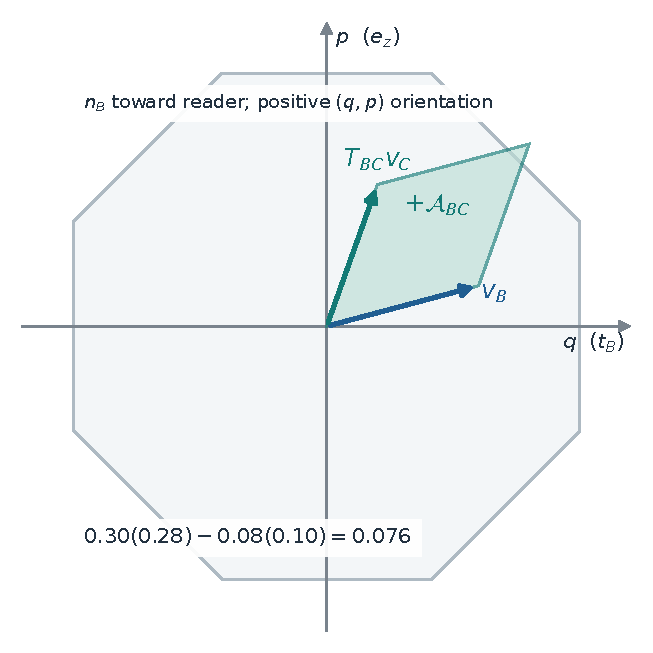
\includegraphics[width=0.72\linewidth,height=\textheight,keepaspectratio,alt={Construction of the transported area in the positively oriented frame at face B. The vectors have coordinates v\_B=(0.30,0.08) and T\_\{BC\}v\_C=(0.10,0.28). The shaded parallelogram has signed area 0.076. The octagon is only a reference carrier; the shaded region is a state-vector construction and is not the physical area of a face.}]{figures/figure_4_signed_area.pdf}
\caption{Construction of the transported area in the positively oriented frame at face B. The vectors have coordinates \(v_B=(0.30,0.08)\) and \(T_{BC}v_C=(0.10,0.28)\). The shaded parallelogram has signed area \(0.076\). The octagon is only a reference carrier; the shaded region is a state-vector construction and is not the physical area of a face.}
\end{figure}

The state amplitudes in this model have no assigned physical units. The area in (15) consequently has squared state-amplitude units, if units are subsequently assigned; it is not the fixed material area of an octagon. The observable retains raw scale. It has no imposed decay envelope; it need not decay. No conservation or monotonicity theorem for \(Z\) follows from (16).

\subsection{7. Transformation laws and their meanings}\label{transformation-laws-and-their-meanings}

There are four operations to distinguish: multiplying the state by a common phase, permuting channel coordinates, actively moving the shell and its tangent vectors, and passively changing the coordinate frames of unchanged vectors. Only after these kinematic actions are defined can one ask whether a specified recurrence commutes with them.

\textbf{Proposition 5 (state-coordinate transformations; exact algebra, inherited from {[}BI, FA{]}).} Common phase leaves \(\mathcal A\) and \(Z\) unchanged, while complex conjugation changes both signs. If \(Q\) is any three-channel permutation matrix and only the channel state is permuted, then
\paperdisplay[17]{\mathcal A(Q\Omega)=Q\mathcal A(\Omega)Q^T,\qquad
Z(Q\Omega)=\det(Q)\,QZ(\Omega).}

\emph{Proof.} The phase and conjugation statements follow immediately from \(\operatorname{Im}(\overline{\Omega_i}\Omega_j)\). Permuting the two indices proves the matrix formula. The cross-product identity
\((Qa)\times(Qb)=\det(Q)Q(a\times b)\) proves the second one. Here the three real axes are channel coordinates. \(\square\)

For a spatial symmetry let \(G\) denote its orthogonal linear part and let \(\pi\) be the induced face permutation, represented by \(Q\). Its point action is \(x\mapsto o+G(x-o)\), whereas its action on face vectors is
\paperdisplay[18]{v'_{\pi(i)}=Gv_i,\qquad n_{\pi(i)}=Gn_i.}
For the present group \(Ge_z=\eta e_z\) with \(\eta=\pm1\). The axial transformation identity for a cross product gives
\paperdisplay[19]{Gt_i=\det(G)\eta\,t_{\pi(i)}.}
Consequently the transformed complex component is
\(\Omega'_{\pi(i)}=\eta\Omega_i\) for \(\det(G)=1\) and
\(\Omega'_{\pi(i)}=-\eta\overline{\Omega_i}\) for \(\det(G)=-1\).
The improper actions are conjugate-linear. This statement concerns the oriented-plane encoding, not an assumed time-reversal operation.

\textbf{Theorem 6 (spatial and channel parity; corrected law from {[}FA, §10{]}, proved here).} For the spatial action (18) of a shell symmetry,
\paperdisplay[20]{\mathcal A'=\det(G)\,Q\mathcal A Q^T,\qquad
Z'=\det(G)\det(Q)\,QZ.}

\emph{Proof.} Equation (19) and \(Ge_z=\eta e_z\) imply
\(GT_{ij}G^T=T_{\pi(i)\pi(j)}\): each outer product acquires the square of a sign. Inserting this covariance and (18) in (15), and using
\((Gv)\times(Gw)=\det(G)G(v\times w)\), gives
\(\mathcal A'_{\pi(i)\pi(j)}=\det(G)\mathcal A_{ij}\).
The first equality follows. Passing from the antisymmetric matrix to its cyclic triple introduces the channel-permutation determinant, as in (17), and proves the second. \(\square\)

Let \(S\) swap \(A\) and \(C\). For the three generators, (20) reads
\paperdisplay[21]{\begin{array}{c|c|c}
\text{spatial action}&\text{state action}&\text{area-triple action}\\ \hline
C_3 & P\Omega & PZ\\
H & \overline\Omega & -Z\\
V & -S\overline\Omega & SZ
\end{array}}
For \(V\), both determinants are negative and cancel. For \(H\), the permutation is the identity and the spatial sign remains. The two signs encode separate facts.

\begin{figure}
\centering
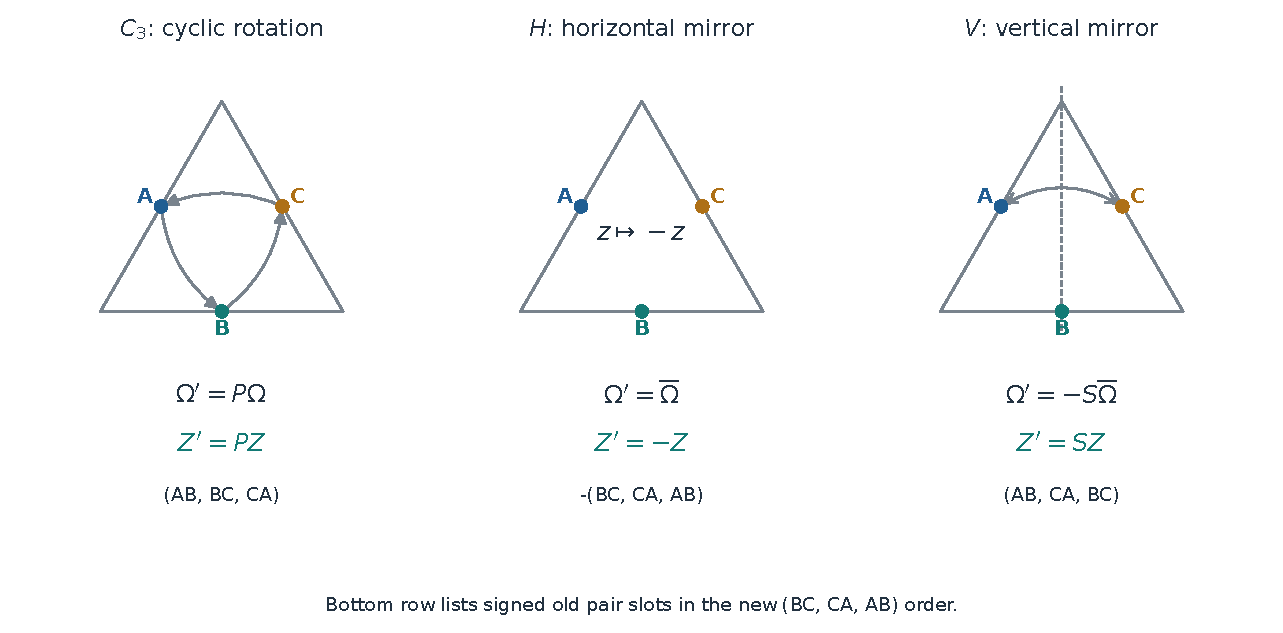
\includegraphics[width=1\linewidth,height=\textheight,keepaspectratio,alt={Generator actions. Upper panels use the exact central-section coordinates to display the face permutation; the horizontal mirror leaves this projection fixed but reverses the vertical component. Lower rows give the actions on the state and on the channel-pair slots Z=(\textbackslash mathcal A\_\{BC\},\textbackslash mathcal A\_\{CA\},\textbackslash mathcal A\_\{AB\})\^{}T. These slot arrows and formulae do not identify Z with an ambient vector.}]{figures/figure_5_symmetry.pdf}
\caption{Generator actions. Upper panels use the exact central-section coordinates to display the face permutation; the horizontal mirror leaves this projection fixed but reverses the vertical component. Lower rows give the actions on the state and on the channel-pair slots \(Z=(\mathcal A_{BC},\mathcal A_{CA},\mathcal A_{AB})^T\). These slot arrows and formulae do not identify \(Z\) with an ambient vector.}
\end{figure}

A passive frame change is different. Rotate the basis at face \(i\) by an angle \(\theta_i\):
\paperdisplay[22]{t'_i=\cos\theta_i\,t_i+\sin\theta_i\,e_z,\qquad
e'_i=-\sin\theta_i\,t_i+\cos\theta_i\,e_z.}
The unchanged vector has new coordinate \(\Omega'_i=e^{-\mathrm i\theta_i}\Omega_i\). If the geometric transport itself is kept fixed, its new coordinate multiplier from \(j\) to \(i\) is \(e^{\mathrm i(\theta_j-\theta_i)}\). The invariant area is then
\paperdisplay[23]{\operatorname{Im}\!\left(
\overline{\Omega'_i}\,e^{\mathrm i(\theta_j-\theta_i)}\Omega'_j
\right)=\mathcal A_{ij}.}
Using the unmodified expression \(\operatorname{Im}(\overline{\Omega'_i}\Omega'_j)\) for independently changed frames would instead reset the transport convention. The real off-diagonal entries in (11) use the original zero-relative-phase frame match. This is why passive covariance is not permission to alter the transport while claiming the same map.

\subsection{8. A channel pseudovector is not an ambient axial vector}\label{a-channel-pseudovector-is-not-an-ambient-axial-vector}

An ambient axial vector \(w\in\mathbb R^3\) transforms under an orthogonal spatial map as \(w'=\det(G)Gw\). In contrast, (20) transforms \(Z\) with the face-permutation representation and an additional determinant. Both outputs may be written as triples of real numbers, but they inhabit different representations.

\textbf{Proposition 7 (explicit cyclic witness; reused from the face-state verification and evaluated exactly here).} Interpreting the three entries of the raw \(Z\) directly as ambient Cartesian components fails even for the proper \(C_3\) rotation.

\emph{Proof.} Take the allowed state \(\Omega=(0,1,\mathrm i)^T\). Then \(a=(0,1,0)^T\), \(b=(0,0,1)^T\) and \(Z=(1,0,0)^T\). Equations (5) and (21) give
\paperdisplay[24]{Z(P\Omega)=PZ=(0,1,0)^T,\qquad
RZ=(-\tfrac12,\tfrac{\sqrt3}{2},0)^T.}
These are unequal; their squared distance is \(2-\sqrt3>0\). A proper spatial rotation would send an ambient axial vector by \(R\), not by \(P\). \(\square\)

This witness rejects the direct Cartesian identification. It does not forbid constructing some separately specified map from channel data to geometric observables, and it makes no claim that abstract representations can never be compared after a change of basis and a stated restriction. Such a construction would require its own definition and covariance analysis. None is part of the raw readout (16).

The normal vectors used in each individual area calculation are ambient geometric objects. Their presence does not make the list of three resulting scalars an ambient vector. This distinction is essential if the word ``chirality'' is used: here it denotes the orientation-sensitive channel observable with the explicit laws (17) and (20).

\subsection{9. Relation to nonlinear triad dynamics}\label{relation-to-nonlinear-triad-dynamics}

The coupling in (11) is the negative combinatorial graph Laplacian on the complete graph \(K_3\). With \(f_0=(1,1,1)^T/\sqrt3\) and \(p_0=f_0f_0^\dagger\),
\paperdisplay[25]{L_3=-3(I-p_0).}
Thus coupling alone annihilates the balanced channel and acts with eigenvalue \(-3\) on the transverse complex two-plane. The graph terminology is standard {[}GR01{]}. This spectral identity does not identify channel coordinates with three directions in ambient space, nor does it determine the nonlinear dynamics of \(Z\).

The pre-synchronization part is permutation covariant when the labelled parameters are carried with the state:
\paperdisplay[26]{F_{\mathrm{TO},\,Qk}(Q\Omega)=QF_{\mathrm{TO},\,k}(\Omega).}
The all-pairs three-node phase step has the same permutation covariance, including its site-independent zero convention, so (26) holds for the full map. At fixed labels, equal \(k_i\) is sufficient for the full permutation symmetry. Unequal values generally break that symmetry; the appropriate statement is joint state/parameter covariance. If \(\varepsilon=0\), \(k\) drops out and this particular restriction is vacuous.

The phase step is equivariant under a common phase when every component entering it is nonzero. With \(\lambda\ne0\), this does not follow globally from the common-phase invariance of the area observable: that invariance is a polynomial identity valid at every state, whereas the phase step involves \(\operatorname{Arg}_0\). At \(\lambda=0\) the phase step is the identity and the common-phase qualification at zero disappears. The same care is required before using a spatial mirror involving a common phase factor as a dynamical symmetry. Equations (20) and (21) are kinematic identities regardless.

One update therefore has a concrete geometric description: a radial on-site increment and transported graph coupling in each selected plane, followed by its prescribed outward-normal phase rotation. No motion of the octagonal panels occurs. The shared geometry controls the interpretation of that update; it does not add a second time evolution. Detailed orbit, stability and covering questions belong to {[}PA{]} and are not needed for the area theorem.

\subsection{10. Mathematical context}\label{mathematical-context}

The construction combines standard structures with a particular set of frames. The identities \(J_i^2=-I\) and \(g_i(J_iv,J_iw)=g_i(v,w)\) are the definition of an orthogonal complex structure. The compatible constant two-form makes each vector plane a flat symplectic and Kähler space. Our sign convention and proof are explicit in (8), and the corrected bridge {[}BII{]} fixes their use here. A precise external textbook locator for this terminology remains to be verified; no unverified reference is being used as a premise.

The matrix \(\mathcal A\) is an alternating bilinear pairing of channel entries after transport. Its cyclic triple is the familiar three-dimensional dual of an antisymmetric matrix in channel space. The determinant in (17) is the usual orientation sign of that dual. The additional spatial determinant in (20) comes from the cross product in an oriented face plane. These are elementary linear-algebra facts applied to two separately specified actions.

The geometric \(C_3\) subgroup and its mirrors use the point-group setting of {[}Cotton90, AH94{]}. The comparison between a network map and its permutation action belongs to the established language of equivariance and synchrony {[}SGP03{]}; that literature is contextual here. No theorem about continuous coupled-cell flows is imported to establish the discrete recurrence. Similarly, {[}GR01{]} supplies graph-Laplacian terminology, while (25) is directly checked. The tangent-space interpretation does not follow from those general references: it depends on the model-specific frames (3), the observable adoption (6), and the transport choice (9).

\subsection{11. Limits of physical interpretation}\label{limits-of-physical-interpretation}

The local result is a mathematical correspondence between a complex state and a geometric observable. The chosen normalization gives the octagon width as one; it supplies no physical length unit and no units for \(\Omega\). No electromagnetic, mechanical or other physical field is recovered by attaching three free vectors to face centres.

The construction supplies neither a seam field law nor continuity of a field on the whole folded surface. It specifies no boundary conditions at the rims and proves no physical mode-selection theorem. Three selected planes give a six-real-dimensional state space by definition; they are not a derivation that an unspecified continuum system has exactly three complex modes.

The finite spatial point group fixes no time scale, physical frequency or temporal phase generator. Phase multiplication has a geometric meaning as a plane rotation, but interpreting it as physical time evolution would require further dynamical input. The nonlinear map is already given and retains its parameter and zero-stratum qualifications.

Finally, the area triple is not identified with magnetism, angular momentum or any other ambient axial quantity. The counterexample in (24) prevents that direct identification. No \(E_6\) or \(E_8\) result is asserted here. These limits identify the extra hypotheses a physical interpretation would need without weakening the exact statements proved above.

\subsection{12. Conclusion}\label{conclusion}

The folded module supplies three outward-oriented tangent planes with canonical frames relative to the chosen vertical direction. They realize a complex triad isometrically, admit a matched transport with exact composition, and express the existing triad recurrence by coordinate conjugacy. The raw chirality readout is precisely a triple of transported signed areas. Its symmetry law separates spatial orientation from channel permutation, and an explicit cyclic witness shows why that triple must not be read as an ambient axial vector. This establishes a controlled geometric interpretation of the local state and its orientation observable within the declared finite-dimensional model.

\subsection{Appendix A. Reproducibility and implementation correspondence}\label{appendix-a.-reproducibility-and-implementation-correspondence}

The accompanying package contains the five figure sources and a bounded symbolic checker. Figure coordinates are generated from (1)-(3) and compared exactly with the accepted geometry implementation before rendering. Plotting converts the resulting exact values to floating-point coordinates; no fitted shell or alternate mesh is used. The algebra checker verifies the displayed identities, not a parameter sweep or a trajectory experiment. The proofs in the text are independent of the number of software tests.

The repository\textquotesingle s \textbf{kernel\_physics} package gives equation-to-code evidence in the modules \textbf{geometry.py}, \textbf{face\_state.py}, \textbf{dynamics.py} and \textbf{readouts.py}. In particular, \textbf{decode\_to\_faces} and \textbf{encode\_from\_faces} implement (6), \textbf{transport} implements (9), and \textbf{z\_chiral} computes the raw cross product in (16). The exact formulae concern real or complex arithmetic; floating-point encoding and decoding are rounded and are not claimed to be bitwise inverses. The implementation rejects substantive normal components and has explicit finite-precision limits.

\textbf{FaceState} retains canonical \(\Omega\) and derives its displayed face vectors. A step calls the selected existing recurrence once on that stored complex state, then decodes its returned value. It does not repeatedly encode the geometric display or evolve a second face state. An explicit initialization from supplied tangent vectors can encode once. This ownership rule prevents the geometric view from changing a trajectory through repeated coordinate-rounding feedback.

Relevant existing files in \textbf{kernel\_physics/tests} are \textbf{test\_face\_state.py}, \textbf{test\_dynamics.py} and \textbf{test\_readouts.py}. They cover exact frames, inverse-domain and projector identities, transport composition, the recurrence dictionary, signed areas, separate spatial and channel signs, parameter/zero qualifications, and canonical-state call ownership. These are implementation checks, not substitute proofs. No user interface is required to reproduce the paper.

The companion symbol/theorem sheet gives the statement-to-source correspondence. The reference ledger records the current versions of the internal technical sources and the inherited external metadata checks. The publication package includes the complete Markdown, generated TeX, figure files and build instructions; these suffice to read the argument without access to earlier discussions.

\subsection{Acknowledgement}\label{acknowledgement}

AI-assisted tools were used in the underlying mathematical reconstruction, verification and manuscript preparation. All scientific claims, interpretations and publication decisions remain the responsibility of the author.

\clearpage

\subsection{References}\label{references}

\textbf{{[}PA{]}} H. F. Halldórsson. \emph{Cycle-Covering Dynamics of a Three-State Nonlinear Kernel}. Project manuscript, v0.5.1, 2026. Relevant source: §6.1, deterministic three-node recurrence and zero convention. See the accompanying reference ledger for the exact source filename.

\textbf{{[}PC{]}} H. F. Halldórsson. \emph{Exact Geometry of the Folded Tri-Octagon Module}. Project manuscript, v0.3.1, 2026. Relevant sources: §§4, 5, 7, 9, exact placement, orientation and symmetry.

\textbf{{[}BI{]}} \emph{First bridge: folded geometry to three complex state components} and \emph{Unresolved Interface Assumptions}. Project technical reports, 2026. Current source versions recorded in the accompanying reference ledger. Used for the tangent-space complex structure and its physical-interpretation limits.

\textbf{{[}BII{]}} \emph{Phase Bridge II: Independent Verification}. Corrected project technical review, 21 September 2026. Used for the compatible metric, complex structure and area-form conventions; later Hamiltonian claims are not needed here.

\textbf{{[}FA{]}} \emph{Folded-Face State Attachment}, v0.1, including the attributed reconciliation, implementation and validation in §10, 23 September 2026. Project technical report.

\textbf{{[}Cotton90{]}} F. A. Cotton. \emph{Chemical Applications of Group Theory}. 3rd ed. Wiley, 1990. ISBN 0-471-51094-7.

\textbf{{[}AH94{]}} S. L. Altmann and P. Herzig. \emph{Point-Group Theory Tables}. Clarendon Press, Oxford, 1994. ISBN 0-19-855226-2.

\textbf{{[}GR01{]}} C. Godsil and G. Royle. \emph{Algebraic Graph Theory}. Graduate Texts in Mathematics 207. Springer, 2001. DOI: \href{https://doi.org/10.1007/978-1-4613-0163-9}{10.1007/978-1-4613-0163-9}.

\textbf{{[}SGP03{]}} I. Stewart, M. Golubitsky and M. Pivato. ``Symmetry groupoids and patterns of synchrony in coupled cell networks.'' \emph{SIAM Journal on Applied Dynamical Systems} 2(4), 609-646, 2003. DOI: \href{https://doi.org/10.1137/S1111111103419896}{10.1137/S1111111103419896}.

\end{document}
